\PassOptionsToPackage{dvipsnames}{xcolor}
\documentclass[aspectratio=169]{beamer}

\mode<presentation> {

\usetheme{Montpellier} 
\usecolortheme{beaver}

\setbeamertemplate{footline}[page number] 
\setbeamertemplate{navigation symbols}{} % To remove the navigation symbols from the bottom of all slides uncomment this line
}

\setbeamertemplate{caption}[numbered]
\setbeamerfont{caption}{size=\scriptsize}
%\usepackage{etex}
\usepackage{array} 
\usepackage{graphicx} % Allows including images
\usepackage{booktabs} % Allows the use of \toprule, \midrule and \bottomrule in tables
\usefonttheme{professionalfonts}
\usepackage{mathptmx}
\usepackage{caption}
\usepackage{subcaption}
\usepackage{amsmath,amsthm,amssymb}
\usepackage{float}
\usepackage{multirow}
% ------------------ My own stuff
\usepackage[utf8]{inputenc}
\usepackage[T1]{fontenc}

\usepackage{amsmath,amsthm,amssymb}

\beamertemplatenavigationsymbolsempty

\usepackage{rotating}
\usepackage{tikz}
\usepackage{fancyvrb}
\usepackage{listings}
\usepackage{verbatim}

\newcommand\blfootnote[1]{%
	\begingroup
	\renewcommand\thefootnote{}\footnote{#1}%
	\addtocounter{footnote}{-1}%
	\endgroup
}


%------------------
%	TITLE PAGE
%------------------

\title[DFTS2 for CI]{DFTS2: Deep Feature Transmission Simulation
\\ for \\ Collaborative Intelligence}
\subtitle{\small VCIP 2021. Paper ID: xxxx} 

\author[Hans]{Ashiv Dhondea, Robert A. Cohen and Ivan V. {Bajić}}% Your name
\institute[SFU-Multimedia Lab] 
{
\small
Multimedia Lab\\School of Engineering Science\\Simon Fraser University. Burnaby, BC. Canada \\ % Your institution for the title page
\smallskip
\centering

\includegraphics[scale=0.23]{SFUhorizontallogorgb.pdf}
}
\date{\today} % Date, can be changed to a custom date

\begin{document}

\begin{frame}
\titlepage % Print the title page as the first slide
\end{frame}

\begin{frame}
\frametitle{Overview} % Table of contents slide, comment this block out to remove it
\tableofcontents % Throughout your presentation, if you choose to use \section{} and \subsection{} commands, these will automatically be printed on this slide as an overview of your presentation
\end{frame}

\section{Collaborative Intelligence}
\begin{frame}
	\frametitle{Introduction: Collaborative Intelligence}
		\begin{figure}
		\begin{minipage}{.48\textwidth}
			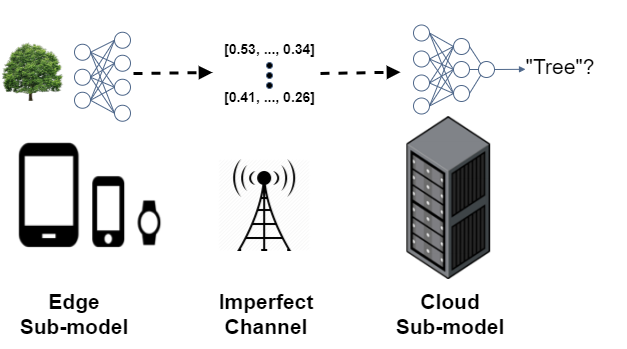
\includegraphics[width=\linewidth]{image--000.png}
			\caption{Blueprint for Collaborative Intelligence. \cite{neurosurgeon}}
		\end{minipage}\hfill
		\begin{minipage}{.48\textwidth}
		\begin{itemize}
		    \item Collaborative Intelligence (CI) leverages edge-based \& cloud-based resources to bring ``AI to the edge". 
		    \item CI has shown promising potential for latency and energy savings compared to purely cloud-based or edge-based analysis solutions \cite{neurosurgeon,jointdnn}.
		\end{itemize}
		\end{minipage}
		\blfootnote{\tiny \textsuperscript{1} Y. Kang, J. Hauswald, C. Gao, A. Rovinski, T. Mudge, J. Mars, and L. Tang, “Neurosurgeon: Collaborative intelligence between the cloud and mobile edge,” SIGARCH Comput. Archit. News, vol. 45, p. 615–629, Apr. 2017.}
		\blfootnote{\tiny \textsuperscript{2} A. E. Eshratifar, M. S. Abrishami, and M. Pedram, “JointDNN: An efficient training and inference engine for intelligent mobile cloud computing services,” IEEE Trans. Mobile Computing, vol. 20, no. 2, pp. 565–576, Feb. 2021.}
	\end{figure}
\end{frame}

\begin{frame}
    	\frametitle{System overview: collaborative intelligence.}
	\begin{figure}[H]
		\centering
		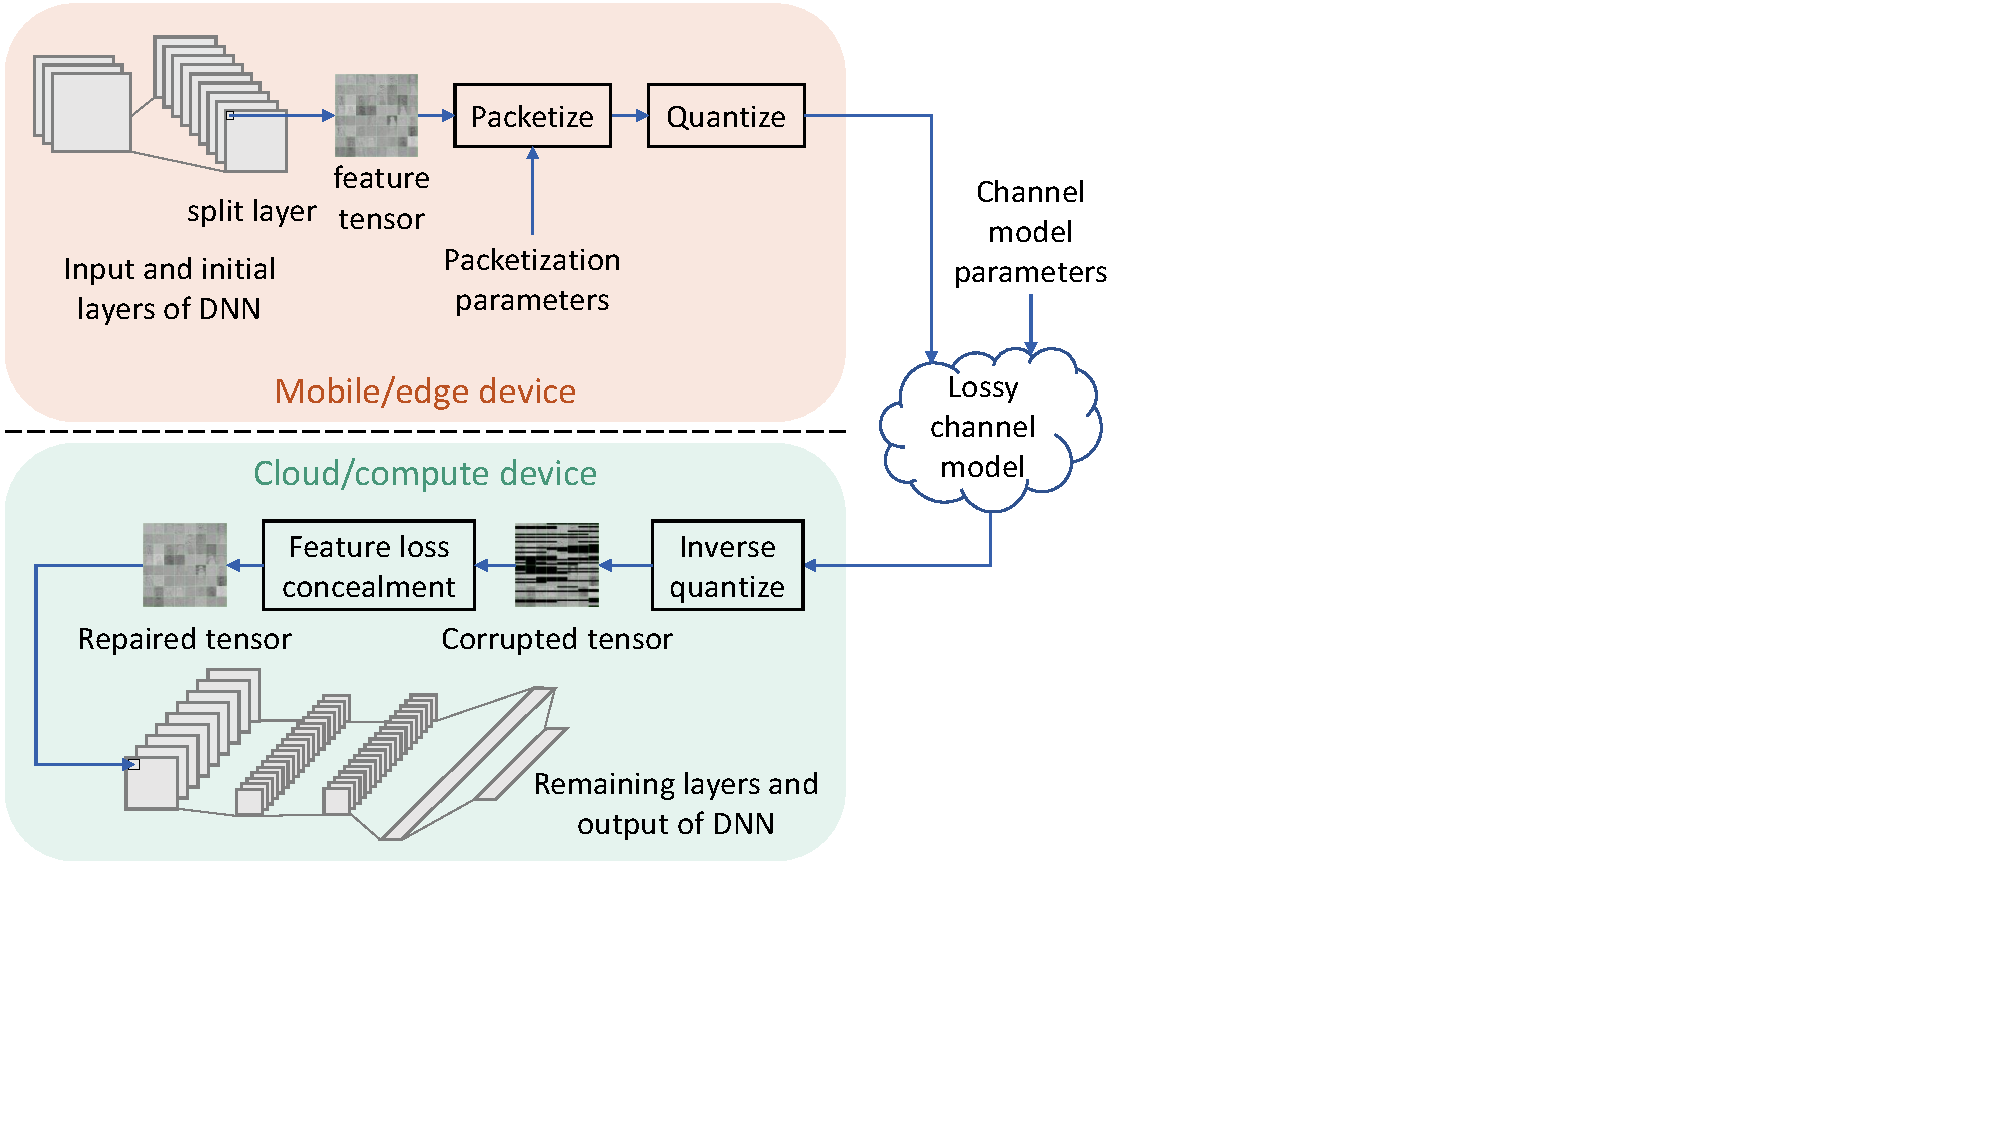
\includegraphics[scale=0.33,viewport=2.391047 126.719996 531.251984 538.217984,clip]{systemoverviewtv3.pdf}
		\caption{Deep feature tensor transmission overview (adapted from \cite[Fig. 1]{cohen2021lightweight})\blfootnote{\tiny \textsuperscript{3} R. A. Cohen, H. Choi, and I. V. Bajić, “Lightweight compression of intermediate neural network features for collaborative intelligence,” IEEE Open Journal of Circuits and Systems, vol. 2, pp. 350–362, 2021.}}
	\end{figure}
\end{frame}

\section{Literature review}

\begin{frame}
\frametitle{Intermediate tensor transmission over communication channels}
	\begin{itemize}
	\item Deep Feature Transmission Simulator (DFTS) was developed to simulate packet-based transmission of deep features over unreliable communication channels \blfootnote{\tiny \textsuperscript{4} H. Unnibhavi, H. Choi, S. R. Alvar, and I. V. Bajić, “Dfts: Deep feature transmission simulator,” 2018.} \cite{unnibhavi2018dfts}.
	\item DFTS2: more sophisticated simulation framework:
	\begin{itemize}
	    \item TensorFlow version 2 compatibility.
	    \item Additional communication channel models and simulation modes.
	    \item Missing feature recovery methods from the literature.
	\end{itemize}
	\item A comprehensive study of packet loss concealment methods on several DNNs.
	\end{itemize}
\end{frame}

\section{Packetization}
\begin{frame}
	\frametitle{Feature tensor in Collaborative Intelligence}
		\begin{figure}[H]
		\centering
		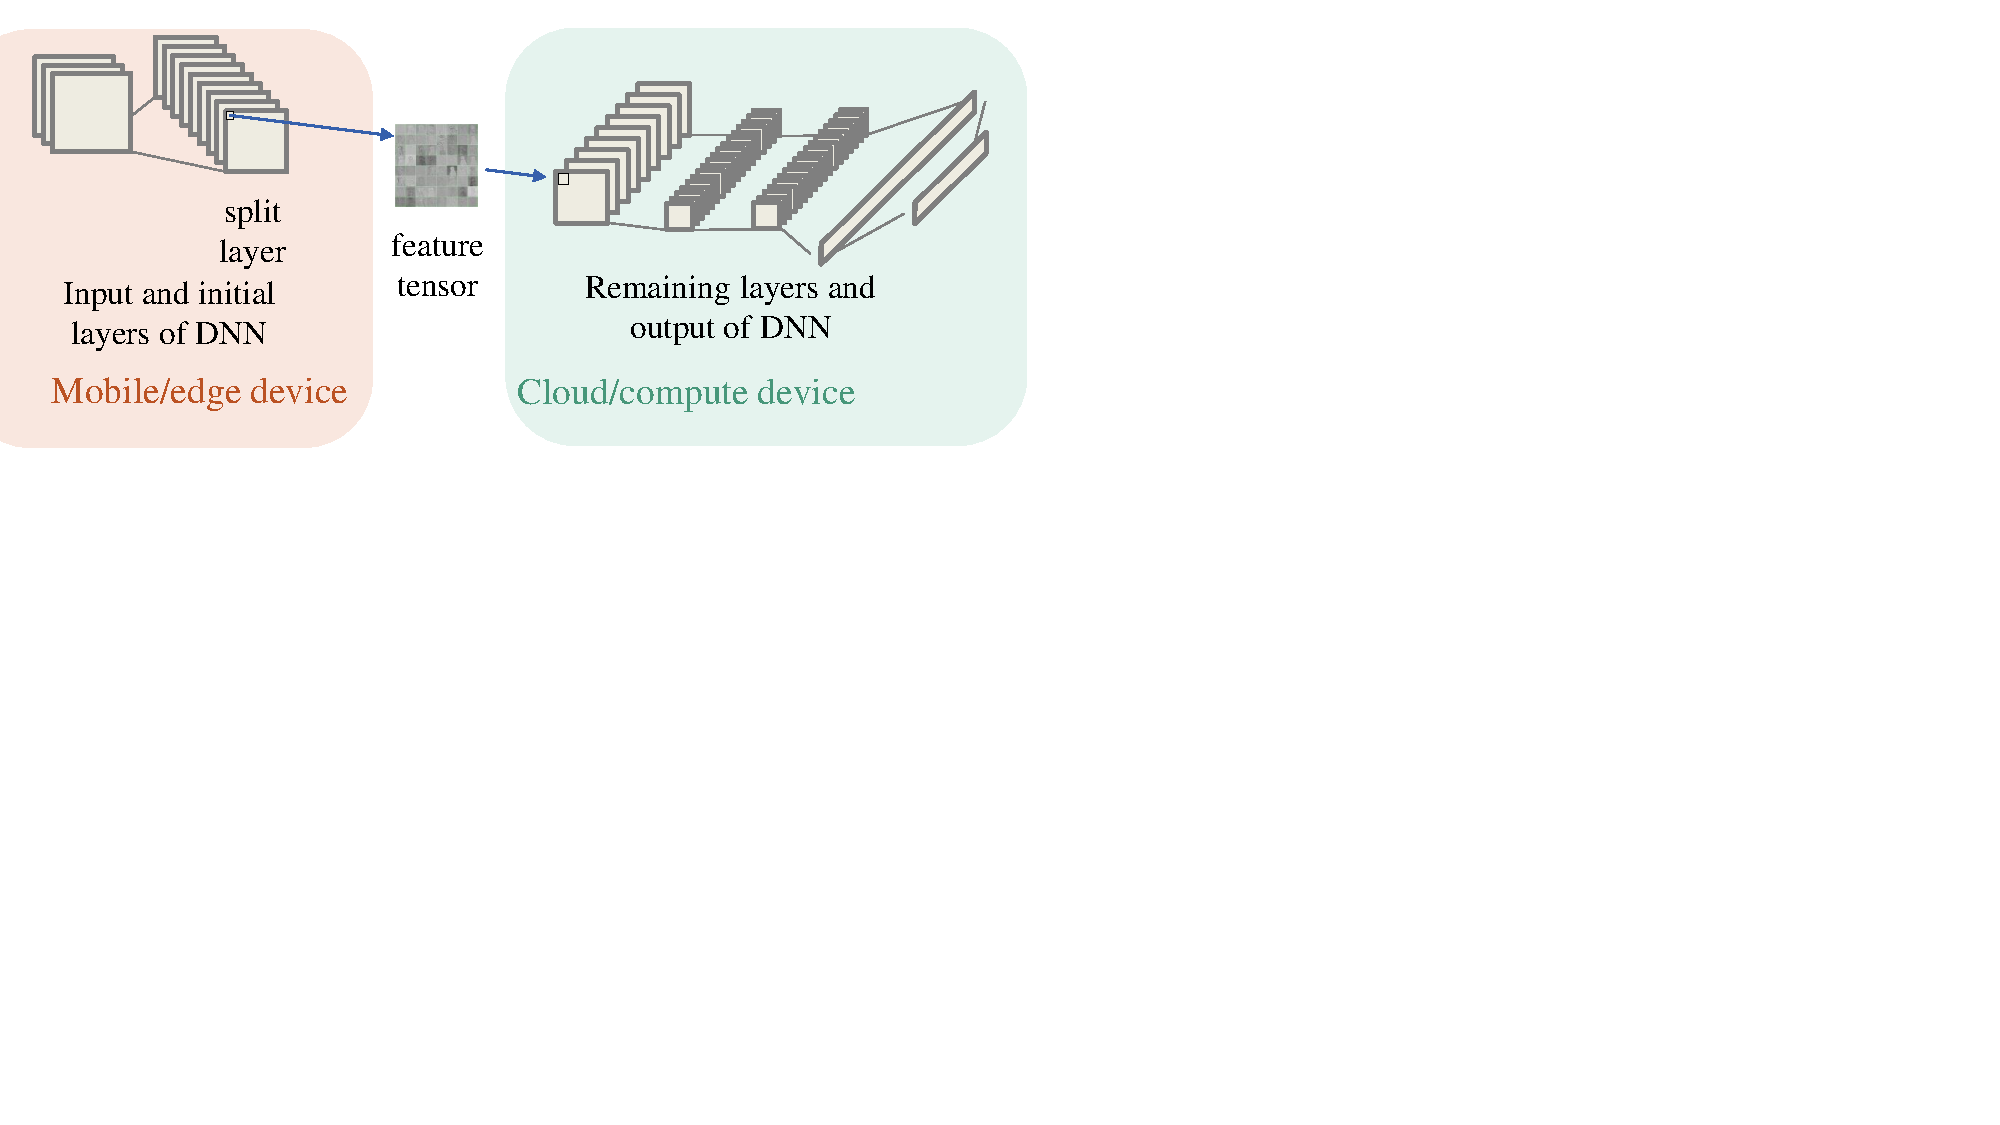
\includegraphics[scale=0.5,viewport=2.391047 296.719996 531.251984 538.217984,clip]{system_overviewt_v4.pdf}
		\caption{Feature tensor in collaborative intelligence (adapted from \cite[Fig. 1]{cohen2021lightweight})\blfootnote{\tiny \textsuperscript{3} R. A. Cohen, H. Choi, and I. V. Bajić, “Lightweight compression of intermediate neural network features for collaborative intelligence,” IEEE Open Journal of Circuits and Systems, vol. 2, pp. 350–362, 2021.}}
	\end{figure}
\end{frame}

\begin{frame}
    \frametitle{Feature tensor packetization}
	\begin{figure}[H]
		\centering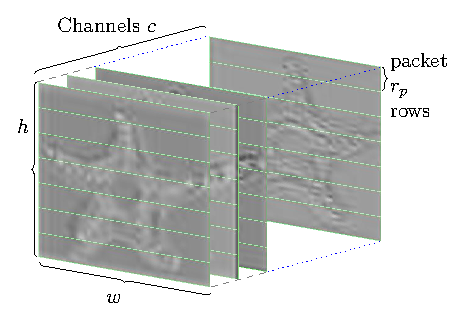
\includegraphics[scale=0.9]{tensorlostviz3icip.pdf}
		\caption{Tensor $\mathcal{X}$ from layer add\_1 of ResNet-18. Several consecutive rows in each channel form a feature data packet.}
	\end{figure}
\end{frame}

\section{Quantization}
\begin{frame}
	\frametitle{Quantizing deep feature tensors}
	\begin{block}{Quantization to $n$-bits}
		For each feature tensor element $x \in \mathcal{X}$
		\[
		x_{\text{quant}} = \Bigg \lfloor \frac{(x - \mathcal{X}_{\text{min}})}{( \mathcal{X}_{\text{max}} -  \mathcal{X}_{\text{min}})} \cdot 2^{n-1} \Bigg \rceil
		\]
		Feature tensors can be cast from 32-bit floats to unsigned 8-bit integers.
	\end{block}
\end{frame}

\begin{frame}
\frametitle{Effect of quantizing deep feature tensors}
    \begin{figure}
        \centering
        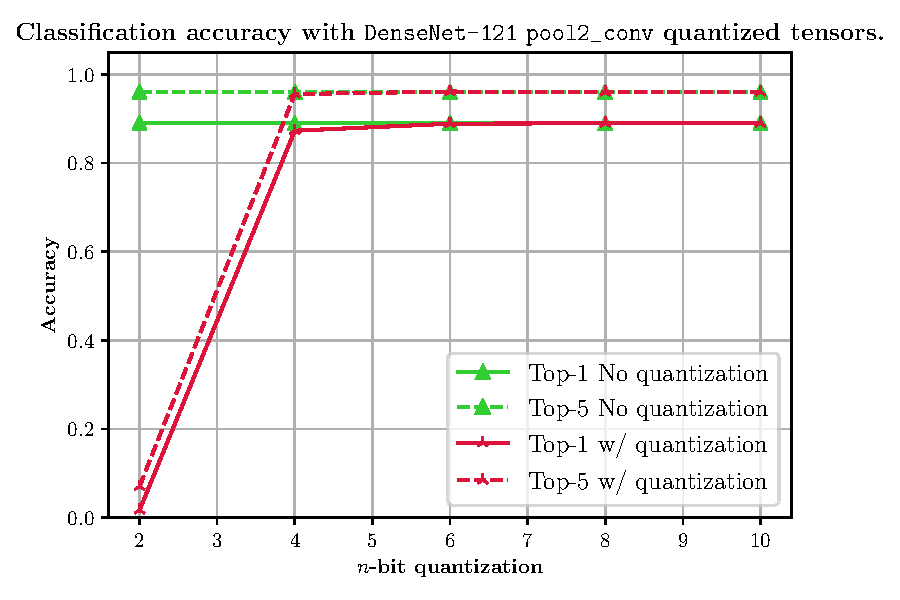
\includegraphics[scale=0.5]{quant_densenet121_pool2_conv.pdf}
        \caption{Classification accuracy on DenseNet-121 pool2\_conv tensors with varying quantization resolution.}
        \label{fig:quant}
    \end{figure}
\end{frame}

\section{Channel models}
\begin{frame}
\frametitle{Communication channel models overview}
\begin{block}{DFTS2 channel models}
\begin{itemize}
    \item An iid (independent and identically distributed) channel model.
	\item Gilbert-Elliott channel model.
	\item External packet traces.
\end{itemize}
\end{block}
\end{frame}

\begin{frame}
\frametitle{Gilbert-Elliott (GE) channel model}
    	\begin{figure}
		\begin{minipage}{.37\textwidth}
		\centering
			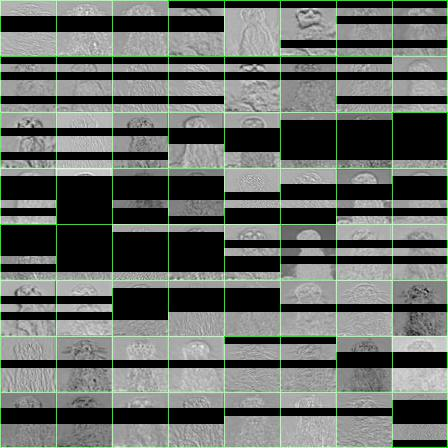
\includegraphics[width=0.8\linewidth]{tileddamagedgridm.jpg}
			\caption{Corrupted ResNet-18 deep feature tensor.}
		\end{minipage}\hfill
		\begin{minipage}{.48\textwidth}
			Two-state Markov model with a good (G) state and a bad (B) state. Parameters: burst loss probability ($P_B$) \& average burst length ($B_L$). \cite{5755057,stuhlmuller2000analysis} 
			\begin{equation}
			\begin{split}
			p_{B\to G} & = \frac{1}{L_B},p_{B\to B} = 1-p_{B\to G}\\
			p_{G\to B} & = \frac{P_B}{L_B(1-P_B)},p_{G\to G} = 1-p_{G\to B}.\\
			\end{split}
			\end{equation} 
		\end{minipage}
	\end{figure}
	\blfootnote{\tiny \textsuperscript{5} G. Hasslinger and O. Hohlfeld, ``The Gilbert-Elliott model for packet loss in realtime services on the Internet,” inProc. 14th GI/ITG Conference - Measurement,Modelling and Evaluation of Computer and Communication Systems, pp. 1–15,2008} \blfootnote{\tiny \textsuperscript{6} K. Stuhlmuller, N. Farber, M. Link, and B. Girod, ``Analysis of video transmission over lossy channels,” IEEE Journal on Selected Areas in Communications, vol. 18,no. 6, pp. 1012–1032, 2000.}
\end{frame}

\begin{frame}
\frametitle{External packet traces}
       \begin{figure}
        \centering
        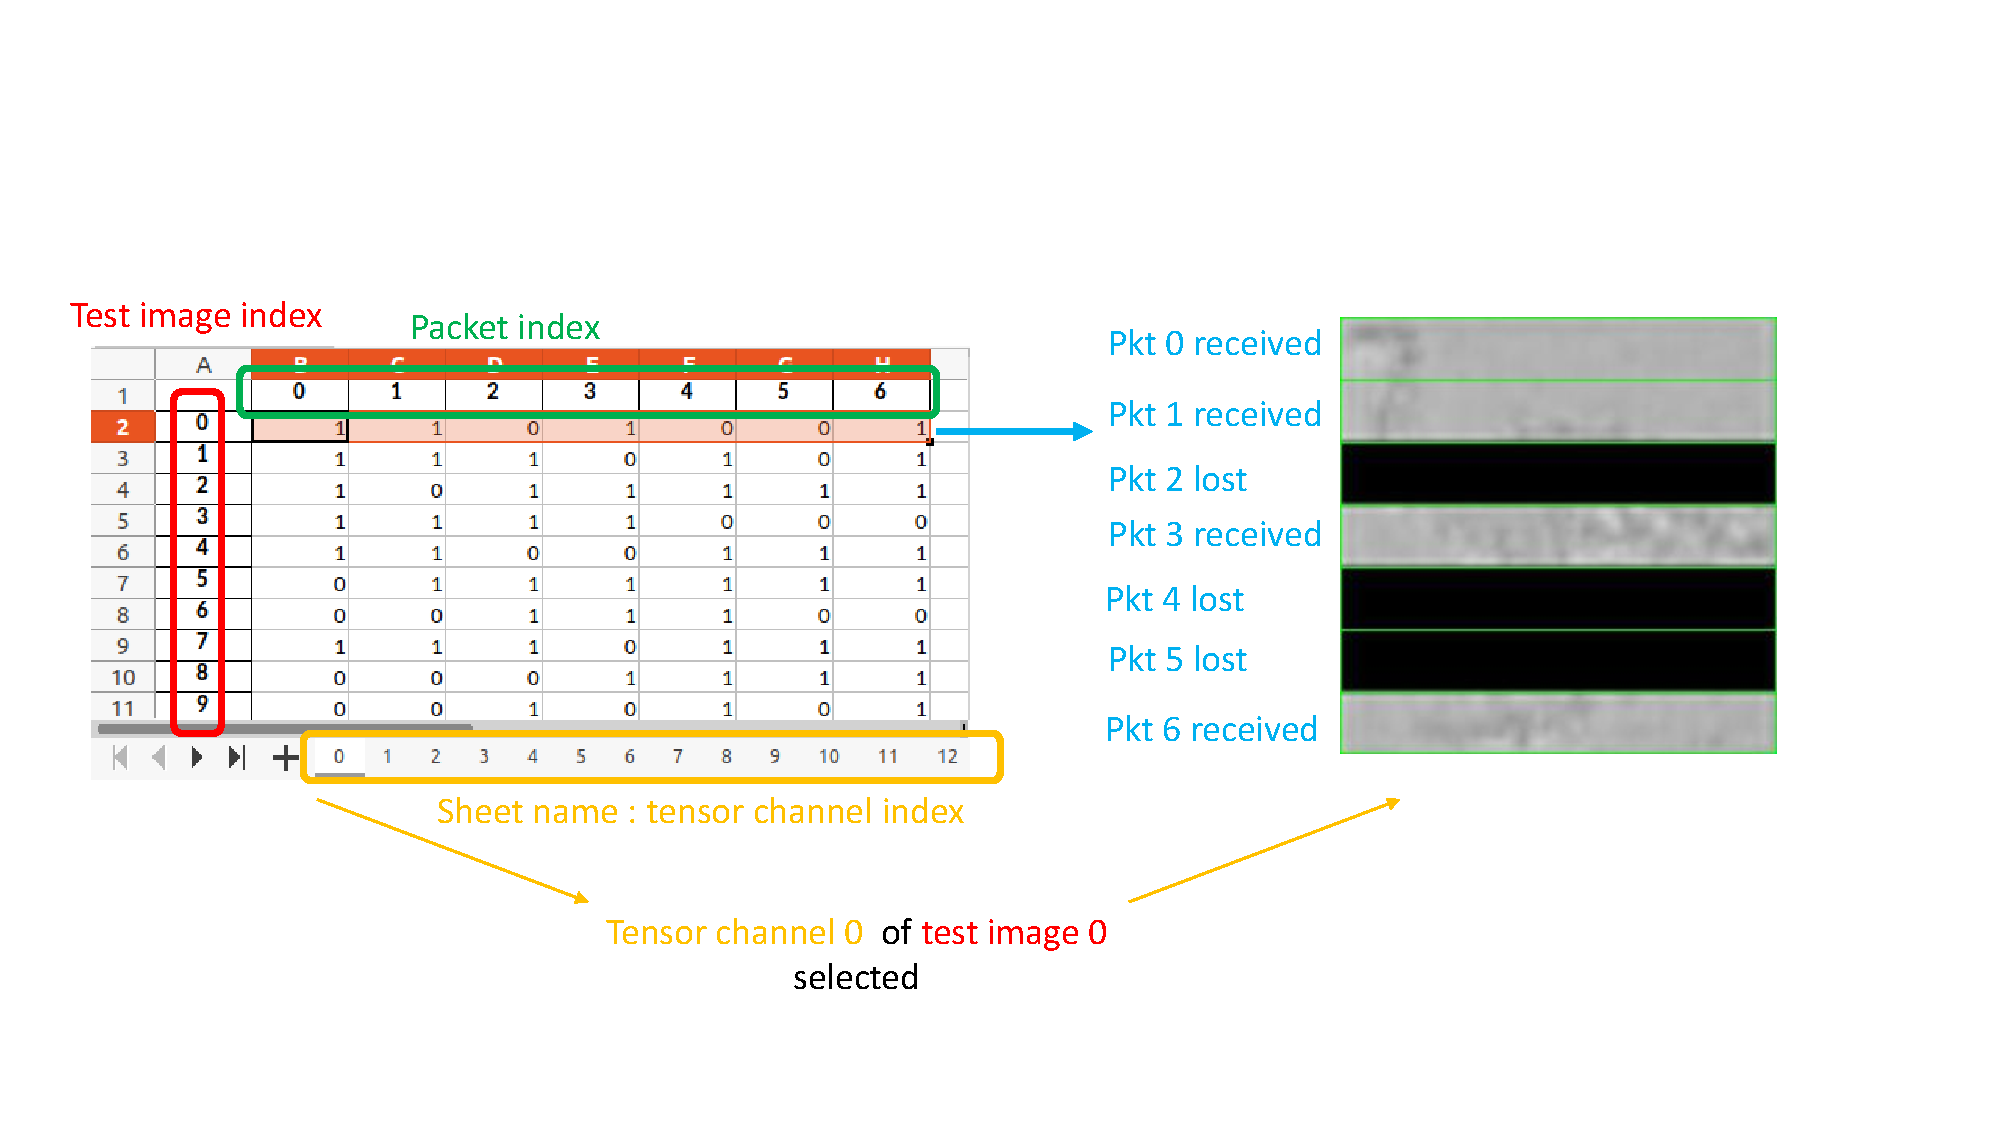
\includegraphics[scale=0.4,viewport=20 60 840 400,clip]{externalpkt.pdf}
        \caption{External packet traces may be captured as Excel files. Each sheet in the Excel file represents a feature tensor channel. Columns represent packet indices within a tensor channel. Rows represent test image indices. A `1' means correctly received packet and a `0' means lost packet.}
        \label{fig:extpkt}
    \end{figure}
\end{frame}

\section{Feature loss concealment}
\begin{frame}
	\frametitle{Packet loss concealment}
	\begin{itemize}
		\item General tensor completion methods, such as SiLRTC (Simple Low Rank Tensor Completion) and HaLRTC (High accuracy Low Rank Tensor Completion) \cite{liu2012tensor}\blfootnote{\tiny \textsuperscript{7} J. Liu, P. Musialski, P. Wonka, and J. Ye,``Tensor completion for estimating missing values in visual data,” IEEE transactions on pattern analysis and machine intelligence, vol. 35, no. 1, pp. 208–220, 2012.}.
		\item Methods tailored for intermediate feature tensors: ALTeC - Adaptive Linear Tensor Completion \cite{Bragile2020} \blfootnote{\tiny \textsuperscript{8} L. Bragilevsky, and I. V.Bajić,``Tensor completion methods for collaborative intelligence,” IEEE Access, vol. 8, pp. 41162–41174, 2020.} and CALTeC - Content-Adaptive Linear Tensor Completion \cite{CALTeC_ICIP_2021} \blfootnote{\tiny \textsuperscript{9} A. Dhondea, R. A. Cohen, and I. V.Bajić, ``CALTeC: Content-adaptive linear tensor completion for collaborative intelligence," Proc. IEEE ICIP, 2021.}
		\item Image inpainting methods such as Navier-Stokes based inpainting \cite{navierstokes} \blfootnote{\tiny \textsuperscript{10} M. Bertalmio, A. L. Bertozzi, and G. Sapiro, ``Navier-Stokes, fluid dynamics, and image and video inpainting,” in Proc. IEEE/CVF CVPR, vol. 1, pp. I–355–I–362, 2001.}
	\end{itemize}
\end{frame}

\section{Simulation modes}
\begin{frame}
\frametitle{Simulation modes}
DFTS2 offers two simulation modes:
	\begin{itemize}
		\item single-shot mode - for demonstration purposes on a small test set.
		\item Monte Carlo mode - for quantitative results in a full-scale experiment.
	\end{itemize}
\end{frame}

\begin{frame}
\frametitle{Demonstration mode}
	\begin{figure}[H]
		\centering
		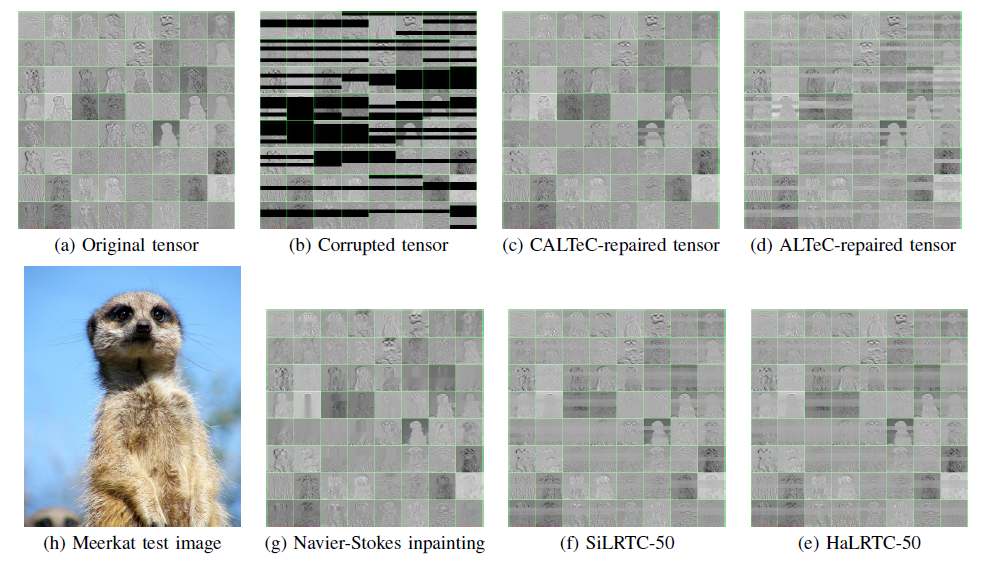
\includegraphics[scale=0.33]{vcipfig.png}
		\caption{Tiled ResNet-34 add\_3 tensor produced from a (h) Meerkat image: (a) original; (b) corrupted; repaired with (c) CALTeC, (d) ALTeC, (e) HaLRTC with 50 iterations, (f) SiLRTC with 50 iterations and (g) Navier-Stokes inpainting. Each tile delineated by green lines represents a channel in a feature tensor. Images were mapped to grayscale for enhanced visualization.}
	\end{figure}
\end{frame}

\begin{frame}
\frametitle{Monte Carlo experiments}
    \begin{table}[t]   \caption{Monte Carlo experiment parameters}
  %\vspace{4pt}
  \label{tab:description:mc}
  \centering
 \begin{tabular}{ l | l }
 %\hline
   \textbf{Component} & \textbf{Parameters} \\
      \hline
      \hline
      \textbf{Model} & ResNet-18, ResNet-34, DenseNet-121 \& EfficientNet-B0. \\
      \hline  
      \textbf{Quantization} & Uniform 8-bit \\
      \hline
      \textbf{Packetization} & 4 or 8 feature rows/ packet (depending on tensor dimensions) \\
      \hline
      \textbf{Channel model} & Gilbert-Elliott ($P_B = \{0.01,0.10,0.20,0.30\},L_B=\{1,2,\dotsc,7\}$)\\
      \hline
      \textbf{Dataset} & 882 image subset of Imagenet \\
      \hline
      \textbf{Monte Carlo} & 20 channel realizations per $(P_B,L_B)$ pair/test image tensor \\
      \hline
      \textbf{Performance metric} & Top-1 \& Top-5 classification accuracy
    \end{tabular}
\end{table}

\end{frame}


\begin{frame}
	\frametitle{Monte Carlo results}
	
	\begin{figure}[H]
		\centering
		\begin{subfigure}{.275\linewidth}
			\centering
			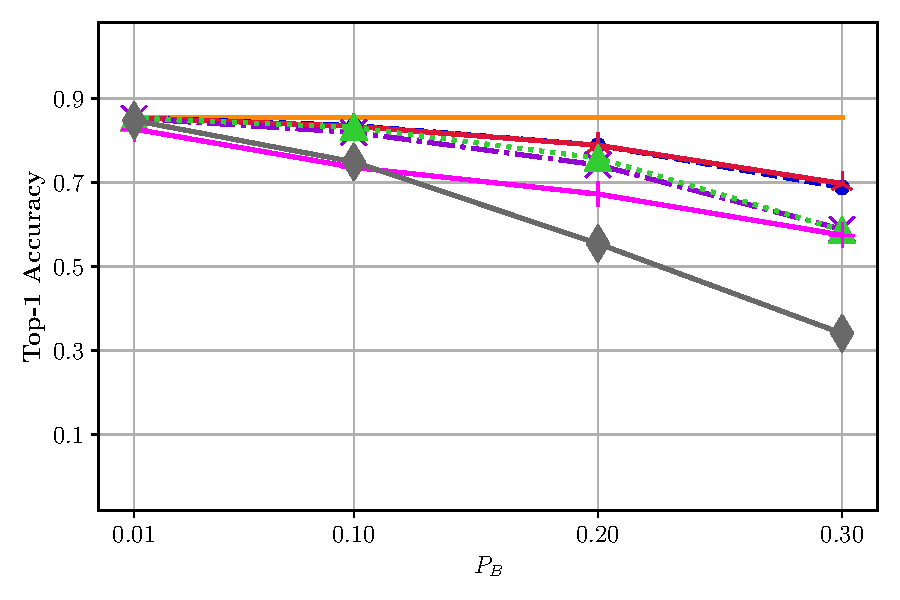
\includegraphics[width = \linewidth]{lp_vcip_rpp_8_top1_resnet18_add_1.pdf}
			\vspace*{-8mm} \caption{ResNet-18 add\_1}
		\end{subfigure}%
		\hfill
		\begin{subfigure}{.275\textwidth}
			\centering
			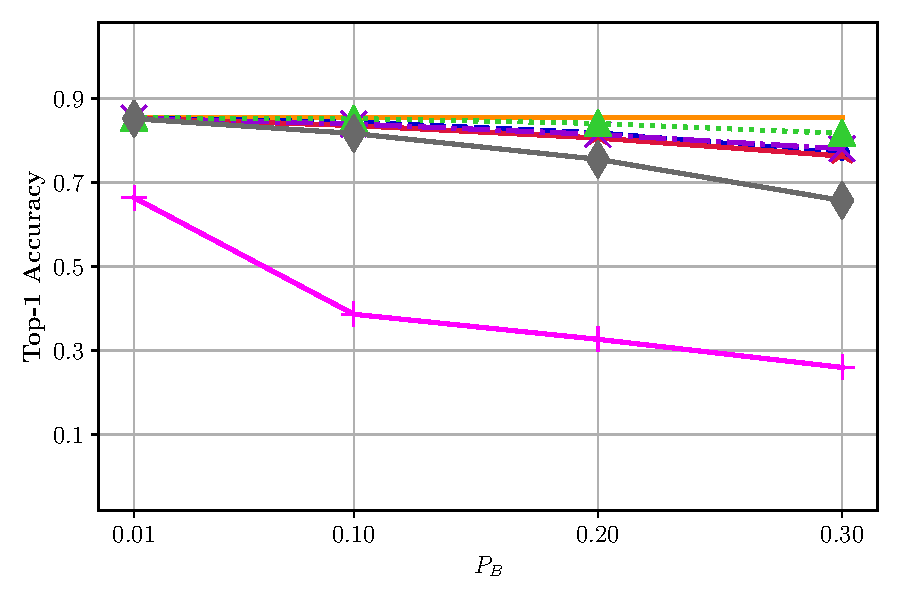
\includegraphics[width = \textwidth]{lp_vcip_rpp_4_top1_resnet18_add_3.pdf}
			\vspace*{-8mm} \caption{ResNet-18 add\_3}
		\end{subfigure}%
		\hfill
		\begin{subfigure}{.275\textwidth}
			\centering
			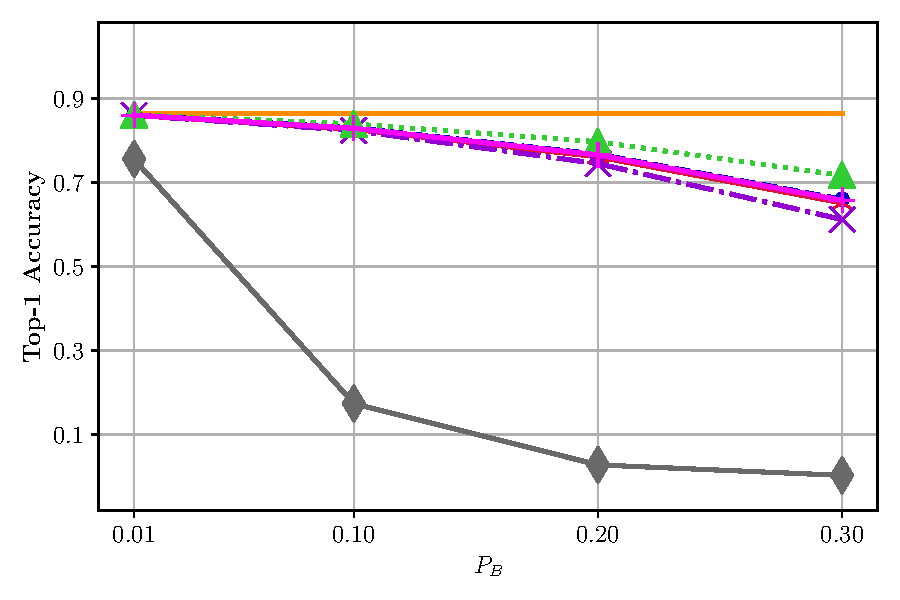
\includegraphics[width=\textwidth]{lp_vcip_rpp_8_top1_efficientnetb0.pdf}
			\vspace*{-8mm} \caption{EfficientNet-B0 block2b\_add}
		\end{subfigure}
		
		\begin{subfigure}{.275\textwidth}
			\centering
			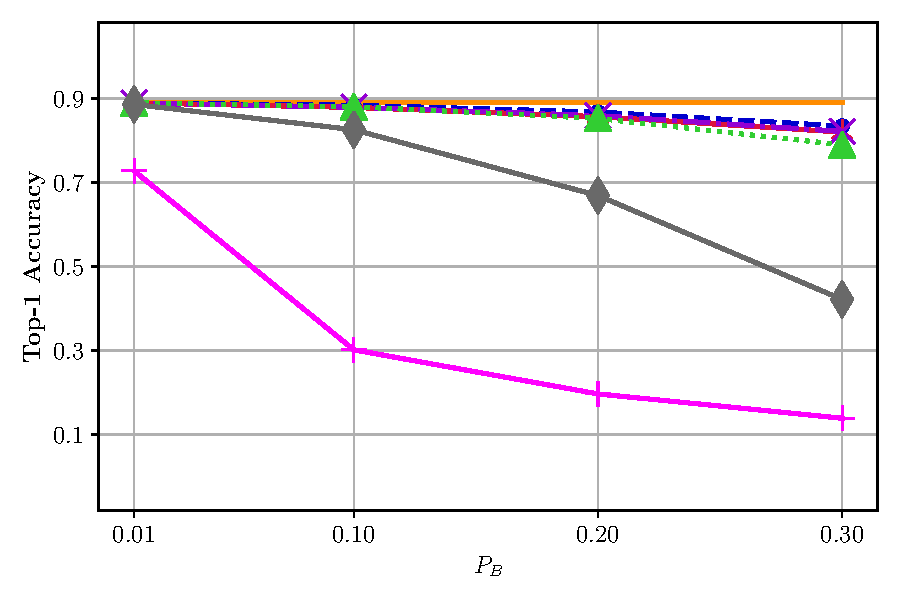
\includegraphics[width = \textwidth]{lp_vcip_rpp_8_top1_densenet121_pool2_conv.pdf}
			\vspace*{-8mm}\caption{DenseNet-121 pool2\_conv}
		\end{subfigure}%
		\hfill 
		\begin{subfigure}{.275\textwidth}
			\centering
			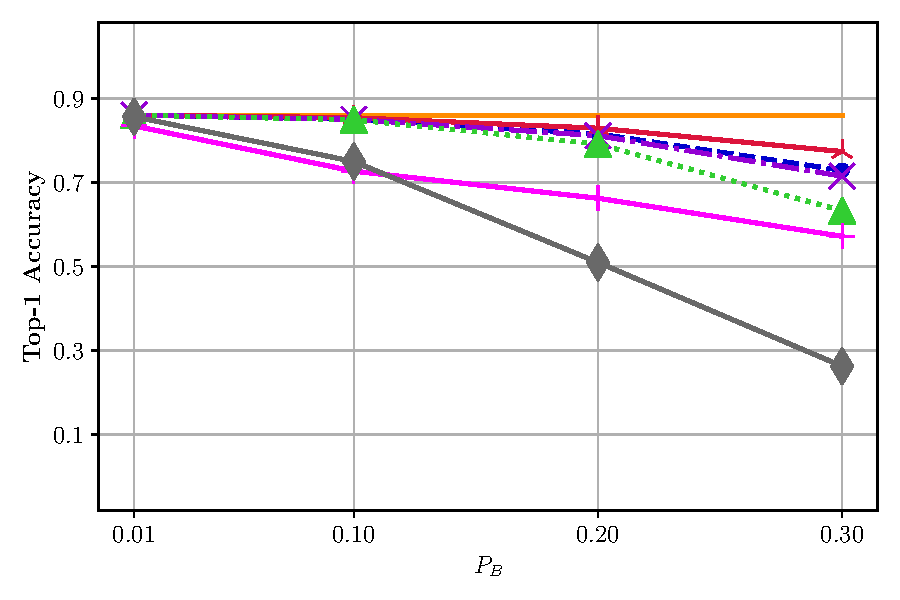
\includegraphics[width=\textwidth]{lp_vcip_rpp_8_top1_resnet34_add_3.pdf}
			\vspace*{-8mm}\caption{ResNet-34 add\_3}
		\end{subfigure}%
		\hfill
		\begin{subfigure}{.275\textwidth}
			\centering
			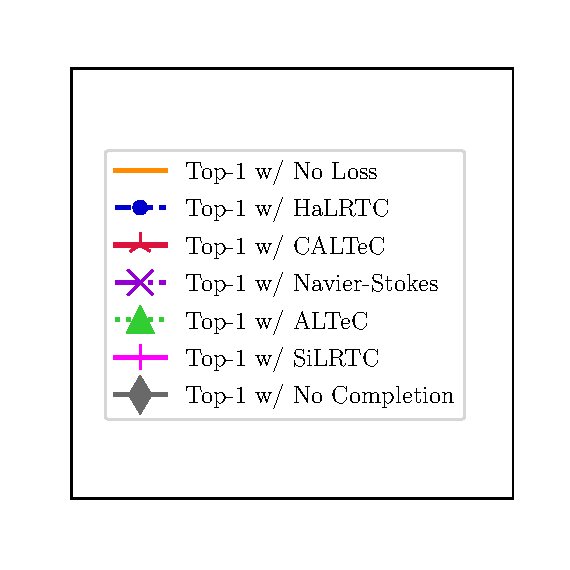
\includegraphics[width=0.9\textwidth]{default_vcip_legend.pdf}
			\vspace*{-6mm}\caption{}
		\end{subfigure}
		\vspace*{-4mm}\caption{Monte Carlo results: Top-1 classification accuracy}
		\label{fig:mc}
	\end{figure}	
\end{frame}


\section{Conclusions}
\begin{frame}
\frametitle{Conclusions}
	\begin{block}{DFTS2}
		More sophisticated framework than DFTS with new capabilities: additional channel models and feature loss concealment.
	\end{block}
\begin{block}{Collaborative image classification}
	A comprehensive study of packet loss concealment methods on several DNNs.
\end{block}
\begin{block}{DFTS2: future work}
\begin{itemize}
    \item Deep feature compression of tensors transmitted over lossy channels in collaborative intelligence.
    \item Additional tasks: collaborative object detection and segmentation.
\end{itemize}
%DFTS2 is flexible: it can be adapted to investigate deep feature compression in collaborative intelligence. DFTS2 is extensible: it can be extended to handle collaborative object detection and segmentation tasks.
\end{block}
\end{frame}

\begin{frame}
\frametitle{Summary of main components of the simulator}
\begin{table}[t]   \caption{Main simulator components}
  %\vspace{4pt}
  \label{tab:description:components}
  \centering
 \begin{tabular}{ l | l }
   \textbf{Component} & \textbf{Options} \\
      \hline
      \hline
      \textbf{Model} & Any tensorflow.keras model \\
      \hline  
      \textbf{Split point} & Any layer \\
      \hline
      \textbf{Quantization} & No quantization or uniform $n$-bit \\
      \hline
      \textbf{Packetization} & $r_p$ feature rows per packet \\
      \hline
      \textbf{Channel model} & Random (iid), Gilbert-Elliott or packet traces    \\
      \hline
      \multirow{2}{*}{\textbf{Loss recovery}} & None, SiLRTC~\cite{liu2012tensor}, HaLRTC~\cite{liu2012tensor}, ALTeC~\cite{Bragile2020}, \\ & CALTeC~\cite{CALTeC_ICIP_2021} or Navier-Stokes~\cite{navierstokes}\\
      \hline
      \textbf{Mode} & Single-shot (demo) or Monte Carlo\\ 
      \hline
    \end{tabular}
\end{table}
\end{frame}

%------------------------------------------------
\section{Implementation}
\begin{frame}
\frametitle{Implementation \& Results}
Public repository for DFTS2: \url{https://github.com/AshivDhondea/DFTS2}.
	\begin{figure}
		\begin{minipage}{.4\textwidth}
			
\includegraphics[width=0.8\linewidth]{qrcode_dpbx.pdf}
			\caption{Source code \& Monte Carlo packet traces and results.}
		\end{minipage}\hfill
		\begin{minipage}{.4\textwidth}
			
\includegraphics[width=0.8\linewidth]{qrcode_github.pdf}
			\caption{GitHub repository \& user documentation}
		\end{minipage}
	\end{figure}
	\end{frame}
	
%---------------------------------------------
\section{References}
\bibliographystyle{ieeetr}
\bibliography{vcipcaltecrefs}
%-----------------------------------------------
\end{document} 